\section{Experiments}
\label{sec:experiments}

We evaluate \ours for the three properties it is designed for. Accuracy is
measured for user memory on conversational recall, document QA, and
personalized generation (\Cref{sec:exp-user}), which mainly exercise semantic
memory together with the episodic records that ground it, and for agent memory
on held-out interactive tasks and on
MetaClaw-Bench, whose tasks span 30 days (\Cref{sec:exp-agent}), which exercise procedural memory. Efficiency is measured
as ingestion time, answer latency, and answer tokens for user memory, with
AutoDream disabled in every timed run, and as training and test tokens for
agents (\Cref{sec:exp-efficiency}). Practicality is built into the protocol itself. One system serves both uses, no model is fine-tuned, the agent
evaluation covers closed and open backbones, and every graph configuration runs
under the budgets of \Cref{sec:retrieval}.

\subsection{Experimental setup and system variants}
\label{sec:exp-setup}

\paragraph{Default system and ablations.}
Unless a configuration is explicitly identified otherwise, \ours denotes the
full architecture with the provenance hypergraph and AutoDream enabled.
For the user-memory ablations, \textbf{M0} uses flat vector memory without the
graph or AutoDream, like MIRIX-1.0~\citep{mirix}, and the tables label it
MIRIX-1.0. \textbf{M1} adds graph indexing and retrieval but disables
AutoDream, and \textbf{M2} is the full graph plus AutoDream configuration.
M1 and M2 are configurations of \ours, not successive releases of the
method. In M2, semantic AutoDream is invoked by the ingestion driver after
every five chunks and after the final chunk, outside the critical write path (Section~\ref{sec:autodream} and \Cref{app:method-autodream}). It merges eligible entity anchors while preserving
stored records and episodic occurrences.

The conversational tables report all three configurations. The available
document QA results and graph efficiency measurements use M1 and are labeled
accordingly; disabling AutoDream there is an experimental choice, not a
restriction that prevents consolidation of document memories. MemoryCD is
reported under the system name, but its recorded results do not identify an
M0, M1, or M2 configuration, so we do not use them to estimate the contribution
of AutoDream. For agent memory, we evaluate the procedural refinement path,
in which AutoDream distills sessions into reusable skills whose retrieval is
independent of the semantic hypergraph. The M0, M1, and M2 comparisons below
therefore concern user-memory indexing and semantic consolidation, rather
than a procedural graph ablation.

\paragraph{User-memory tasks and baselines.}
LoCoMo~\citep{locomo} and LongMemEval-S~\citep{longmemeval} test conversational
recall. SHDocQA, MHDocQA, and DetectiveQA in the MemoryAgentBench
evaluation~\citep{memoryagentbench} extend this analysis to factual and
relational evidence in documents. They are evidence-retrieval tests rather
than direct personalization tasks. MemoryCD~\citep{memorycd} tests whether
stored user information supports personalized review summarization and
generation. We compare with mem0, A-Mem, MemoryBank, Graphiti, and HyperMem on
QA, and with the methods listed in the MemoryCD tables, including
long-context and RAG baselines, on personalization.

\paragraph{Models and scoring.}
For the user-memory evaluation, the answerer and extractor use
\texttt{gpt-4.1-mini} with temperature 0 and seed 42, and the topic extractor
uses \texttt{gpt-4.1-nano}. \ours uses \texttt{text-embedding-3-small}; external
baselines retain their default embeddings. SHDocQA and MHDocQA use substring
matching, and DetectiveQA uses letter exact matching. LoCoMo and LongMemEval-S
use a \texttt{gpt-4o-mini} judge with majority-of-3 voting. MemoryCD uses
ROUGE-1, ROUGE-L, BLEU-4, and BERTScore-F1. Agent backbones and evaluation
protocols are specified in Section~\ref{sec:exp-agent}. Differences in accuracy
or success rate are reported in percentage points.

\paragraph{Efficiency and uncertainty.}
We report total ingestion wall-clock time, mean time to retrieve and answer a
question, total answer tokens, and graph node and edge counts where available.
Graph size measures index structure, not stored text length or total storage.
For interactive agents, we report success, action steps, and training and test
tokens, with mean and standard deviation over three runs. For LoCoMo, all
comparisons below use the results in Table~\ref{tab:locomo}; M0, M1, and M2
are distinct system configurations, not repeated runs used to estimate
variance.

\subsection{User memory: recall, documents, and personalization}
\label{sec:exp-user}

% [24] = narrow lines, one past the caption so the text below it has room; change it if the caption gets longer or shorter
\begin{wrapfigure}[24]{r}{0.49\textwidth}
\vspace{-1.1\baselineskip}
\centering
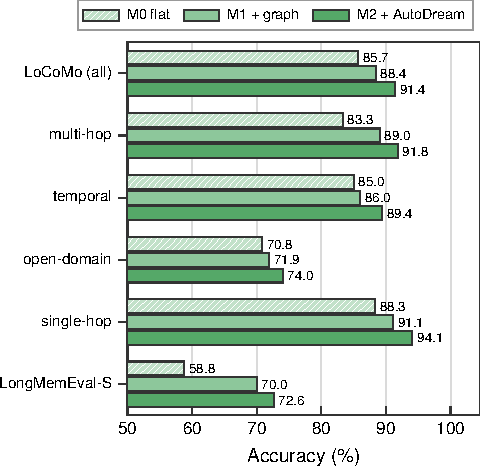
\includegraphics[width=\linewidth]{figures/results_user_ablation.pdf}
\caption{Components of \ours on LoCoMo, its four question types, and LongMemEval-S. The hypergraph (M1) and AutoDream (M2) each add accuracy over flat memory (M0).}
\label{fig:res-ablation}
\vspace{0.3\baselineskip}
\end{wrapfigure}
\paragraph{The hypergraph and AutoDream each improve conversational recall.}
\Cref{fig:res-ablation} and \Cref{tab:locomo}, with \Cref{tab:lme} in the appendix, compare the M0,
M1, and M2 configurations under the evaluation protocol described above and show a
consistent ordering on both conversational benchmarks. On LoCoMo, graph retrieval raises overall accuracy
from 85.7\% for M0 to 88.4\% for M1, and semantic AutoDream raises it to
91.4\% for M2. On LongMemEval-S, the corresponding values are 58.8\%, 70.0\%,
and 72.6\%. The graph increment is thus 2.7 points on LoCoMo and 11.2 points
on LongMemEval-S, while AutoDream adds 3.0 and 2.6 points, respectively.
The larger graph increment on LongMemEval-S suggests that evidence organization
can matter more when flat retrieval has difficulty recovering the relevant
history. It does not establish which question types account for that gain,
since a LongMemEval-S category breakdown is not available here.


\begin{table*}[t]
\centering
\caption{LoCoMo accuracy (\%) by question type on 1{,}540 non-adversarial questions. Bold marks the best value in each column.}
\label{tab:locomo}
\small
\begin{tabular}{lccccc}
\toprule
Method & Overall & Multi-hop & Temporal & Open & Single-hop \\
\midrule
mem0        & 82.9 & 80.5 & 80.4 & 66.7 & 86.6 \\
A-Mem       & 68.3 & 68.8 & 55.5 & 61.5 & 73.8 \\
MemoryBank  & 59.5 & 70.9 & 14.6 & 52.1 & 73.6 \\
Graphiti    & 58.4 & 65.2 & 37.1 & 53.1 & 64.9 \\
HyperMem    & 91.0 & 91.1 & 84.4 & \textbf{76.0} & \textbf{95.2} \\
\midrule
MIRIX-1.0 (M0)                & 85.7 & 83.3 & 85.0 & 70.8 & 88.3 \\
\ours\ (M1, graph)             & 88.4 & 89.0 & 86.0 & 71.9 & 91.1 \\
\ours\ (M2, graph $+$ dream)   & \textbf{91.4} & \textbf{91.8} & \textbf{89.4} & 74.0 & 94.1 \\
\bottomrule
\end{tabular}
\end{table*}
\paragraph{Semantic consolidation can help temporal recall without rewriting events.}
The LoCoMo breakdown is more informative than overall accuracy alone. Moving
from M0 to M1 improves multi-hop accuracy by 5.7 points, compared with 1.0
point on temporal questions. Moving from M1 to M2 then improves every
reported category, including 3.4 points on temporal questions. This pattern is
consistent with the division of work in the method. N-ary frames connect
related evidence, while identity consolidation gives retrieval a more coherent
entry point into records that mention the same entity. Since semantic
AutoDream preserves fact nodes and episodic occurrences, temporal evidence can
become easier to reach without collapsing distinct events. This is an
interpretation of the aggregate results; a direct audit of retrieved records
and merged anchors would be needed to establish the mechanism for individual
answers.

\vspace{4.5pt}% room between the full-width line above and Figure 5
% [17] = narrow lines, one past the caption so the text below it has room; change it if the caption gets longer or shorter
\begin{wrapfigure}[17]{l}{0.49\textwidth}
\vspace{-1.1\baselineskip}
\centering
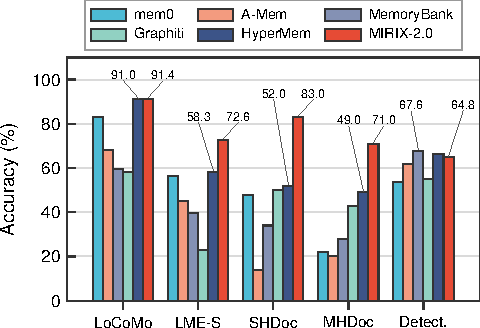
\includegraphics[width=\linewidth]{figures/results_user_baselines.pdf}
\caption{\ours against memory baselines on five QA benchmarks. The document tasks use M1.}
\label{fig:res-baselines}
\vspace{-0.6\baselineskip}
\end{wrapfigure}
\Cref{fig:res-baselines} compares \ours with all memory baselines on the five QA benchmarks. M2
exceeds HyperMem by 0.4 points overall on LoCoMo and by 14.3 points on
LongMemEval-S. Its LoCoMo advantage is concentrated in temporal and multi-hop
questions, with gains of 5.0 and 0.7 points, while HyperMem retains higher
open-domain and single-hop scores. The evidence therefore supports stronger
recovery of connected and time-grounded facts, rather than dominance on every
form of recall. HyperMem's 91.0\% comes from our own run and is lower than the
92.7\% it reports. \Cref{app:results-user} describes how we ran HyperMem with
its original settings.

\paragraph{Keeping source details improves document QA.}
\Cref{tab:docqa} in the appendix reports M1 on document QA. Its 83.0\% on SHDocQA and
71.0\% on MHDocQA exceed HyperMem by 31.0 and 22.0 points. Gains on both tasks
are consistent with a design that retains source details as well as relational structure. Single-hop questions require the precise fact, while multi-hop
questions also require connections between supporting records. In
Sections~\ref{sec:typed-evidence} and~\ref{sec:retrieval}, these requirements
motivate source-faithful writers and retrieval of original rows alongside
graph facts. The comparison measures the combined pipeline and does not
isolate either feature.

DetectiveQA exposes a boundary of this advantage. M1 reaches 64.8\%, below
MemoryBank's 67.6\% and HyperMem's 66.2\%. Organizing explicit evidence does
not by itself guarantee the inference needed to resolve a detective question.
Without an error analysis, we cannot distinguish missed evidence from failures
to reason over retrieved evidence. The document results also cannot establish
an AutoDream benefit, because they evaluate M1 only.
\paragraph{Selective user memory supports personalized generation.}
\Cref{tab:memcd-summ}, and \Cref{tab:memcd-gen} in the appendix, move from answering factual
questions to generating text for a particular user. Cross-domain evaluation is especially relevant because useful preferences must transfer from other product
domains to Home\_and\_Kitchen. This tests a different role for semantic memory
from recalling a named event. A useful record must preserve a user's relevant
preferences while remaining accessible when the new request has a different
surface topic.

For cross-domain summarization, \ours has the highest value on all four
metrics. Its ROUGE-L is .1510, compared with .1430 for the strongest baseline
on that metric, and its BLEU-4 is .0209, compared with .0162. In the
single-domain setting it leads on ROUGE-1 and ROUGE-L and ties the highest
BERTScore, while long-context input has higher BLEU-4. Review generation
shows the highest reported scores for \ours in both settings on all four
metrics, although several margins are small. Together, these results suggest
that selective user memory can preserve useful information for generation
without requiring the full history as context. They do not measure factual
consistency, preference satisfaction, or user approval directly, and the
available configuration record does not support a MemoryCD-specific claim
about graph or AutoDream gains.

\begin{table*}[t]
\centering
\caption{Review summarization on MemoryCD (100 Home\_and\_Kitchen users). Bold marks column maxima.}
\label{tab:memcd-summ}
\small
\begin{tabular}{lcccc|cccc}
\toprule
& \multicolumn{4}{c|}{Cross-domain} & \multicolumn{4}{c}{Single-domain} \\
\cmidrule(lr){2-5}\cmidrule(lr){6-9}
Method & R-1 & R-L & B-4 & BERT & R-1 & R-L & B-4 & BERT \\
\midrule
Long-context & .1493 & .1357 & .0162 & .8745 & .1675 & .1570 & \textbf{.0249} & \textbf{.8779} \\
RAG          & .1559 & .1430 & .0145 & .8735 & .1670 & .1523 & .0196 & .8759 \\
mem0         & .1526 & .1420 & .0159 & .8749 & .1593 & .1472 & .0184 & .8767 \\
A-Mem        & .1567 & .1428 & .0160 & .8746 & .1602 & .1521 & .0184 & .8764 \\
MemoryBank   & .1409 & .1291 & .0131 & .8736 & .1584 & .1449 & .0188 & .8760 \\
Graphiti     & .1534 & .1415 & .0139 & .8741 & .1520 & .1418 & .0172 & .8746 \\
\ours\  & \textbf{.1603} & \textbf{.1510} & \textbf{.0209} & \textbf{.8754} & \textbf{.1715} & \textbf{.1617} & .0234 & \textbf{.8779} \\
\bottomrule
\end{tabular}
\end{table*}


\subsection{Agent memory: held-out tasks and skills}
\label{sec:exp-agent}

\paragraph{Setup and transfer to held-out tasks.}
We evaluate procedural memory on ALFWorld~\citep{shridhar2021alfworld} and
WebShop~\citep{yao2022webshop}, comparing an agent without memory with
ReasoningBank~\citep{ouyang2026reasoningbank}, Agent Workflow Memory
(AWM)~\citep{wang2025awm}, and \ours. Within each comparison, methods share the
actor prompt and backbone. ALFWorld uses GPT-6 Luna and GPT-5.6 Luna; WebShop
uses GPT-6 Luna. Each memory method learns from the same training tasks,
39 for ALFWorld and 40 for WebShop. Memory is then frozen for evaluation on
134 held-out ALFWorld episodes with a 50-step cap and 140 WebShop instructions
with a 15-step cap. Results are averaged over three independent runs.
The separation between memory learning and evaluation tests reuse of acquired
procedures on new tasks.

This setting exercises the procedural branch of AutoDream
(Section~\ref{sec:autodream}). Sessions supply lessons to reuse and mistakes to
avoid, and a curator turns those experiences into skills. Unlike semantic
consolidation, which preserves the factual records and changes their index,
procedural refinement changes the instructions available to the actor. The
experiments evaluate the utility of that combined process; they do not
separately ablate the outcome judge, experience distiller, or curator.

\begin{wrapfigure}{r}{0.49\textwidth}
\vspace{-1.1\baselineskip}
\centering
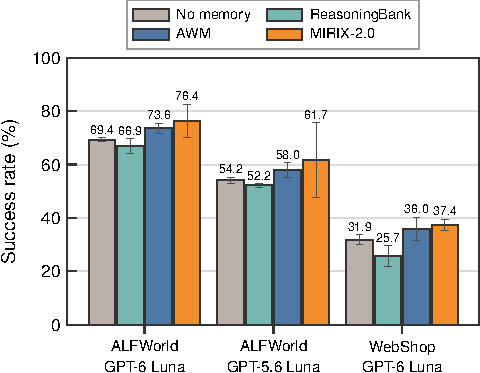
\includegraphics[width=\linewidth]{figures/results_agent_heldout.pdf}
\caption{Agent memory on held-out tasks. Success rate, mean and standard deviation over three runs.}
\label{fig:res-agent}
\vspace{-0.6\baselineskip}
\end{wrapfigure}
\paragraph{ALFWorld: useful procedures must generalize across action sequences.}
\Cref{fig:res-agent}, and \Cref{tab:alfworld-proc} in the appendix, show the highest mean
overall success among the compared methods for \ours with both backbones. With GPT-6 Luna it reaches
76.4\%, compared with 69.4\% without memory and 73.6\% with AWM. With GPT-5.6
Luna it reaches 61.7\%, compared with 54.2\% and 58.0\%, respectively.
The gains over no memory are similar, at 7.0 and 7.5 points, but they are not
uniform across task types (\Cref{fig:res-alfworld-types}). With GPT-6 Luna, Clean improves from 60.2\% to
74.2\% and Heat from 47.8\% to 73.9\%, while Pick, Look, and Pick Two remain
below the no-memory scores. This suggests that procedures are most useful
when they supply missing action structure; retrieving a routine can also
interfere with a task the actor already handles well.

The step counts provide a complementary view. Successful episodes require
13.2 rather than 14.2 steps with GPT-6 Luna and 12.4 rather than 16.1 with
GPT-5.6 Luna, relative to no memory. This is consistent with more direct
action sequences, but the successful subsets differ across methods, so these
are not paired measurements on identical solved tasks. The large success-rate
standard deviations for \ours, 6.2 and 14.0 points, also limit the conclusion. It has the highest observed mean, but three runs do not establish a stable
advantage over AWM.

\paragraph{WebShop: procedure quality matters more than memory availability.}
\Cref{tab:webshop-proc} in the appendix reports 37.4\% success for \ours, compared with
31.9\% without memory, 25.7\% with ReasoningBank, and 36.0\% with AWM.
ReasoningBank falls below no memory on both interactive benchmarks with
GPT-6 Luna, showing that adding experience memory is not sufficient to improve
an actor. In WebShop, \ours leads the memory methods on Fashion and Beauty,
ties AWM on Garden and Grocery, and trails AWM on Electronics. A plausible
interpretation is that reusable constraint checks help some product searches,
while other searches need more task-specific guidance. The category results
do not directly identify which learned skills caused those differences.

\ours uses 8.2 steps per episode and 6.3 per successful episode, fewer than
the other memory methods but slightly more than no memory at 7.9 and 6.2.
Thus, its benefit is a higher success rate with modest additional interaction,
not a reduction in steps relative to every baseline.

\vspace{8pt}% room between the full-width line above and Figure 7
% [18] = narrow lines, one past the caption so the text below it has room; change it if the caption gets longer or shorter
\begin{wrapfigure}[18]{L}{0.49\textwidth}
\vspace{-1.1\baselineskip}
\centering
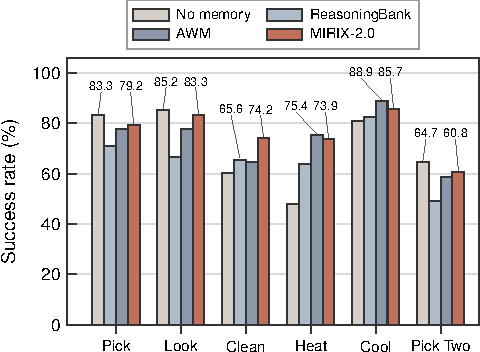
\includegraphics[width=\linewidth]{figures/results_agent_tasks.pdf}
\caption{ALFWorld success by task type with GPT-6 Luna, over three runs.}
\label{fig:res-alfworld-types}
\vspace{-0.6\baselineskip}
\end{wrapfigure}
\paragraph{MetaClaw-Bench: answer quality and completed artifacts are distinct.}
\Cref{tab:metaclaw_part1} evaluates agent memory on Part~I of
MetaClaw-Bench~\citep{xia2026metaclaw}, which spans 30 days.
Accuracy is the official mean
per-question score, which combines binary file checks with partial credit on
multiple-choice questions, and completion is the completion rate over the 224 file-check
questions. With GPT-5.2, \ours improves the official
mean question score from 44.0\% for MetaClaw Skills to 49.2\%, and file-check
completion from 17.1\% to 27.7\%. The larger completion gain, 10.6 points,
suggests that reusable procedures can help produce the required artifacts as
well as improve question scores. With Qwen3.6-35B-A3B, the score gain is
smaller, from 51.8\% to 52.7\%, and completion is tied at 30.8\%. The benefit
therefore depends on the backbone and on what the metric measures.
The GPT-5.2 baselines are reported values from the MetaClaw paper, so this
comparison is not evidence from a fully controlled rerun. Unlike ALFWorld and
WebShop, this table does not report variation across independent runs or a
matched procedural-component ablation.

\begin{table}[tb]
\centering
\captionsetup{justification=centering}
\caption{Agent memory on MetaClaw-Bench Part~I (346 questions).}
\label{tab:metaclaw_part1}
\small
\begin{tabular}{llcc}
\toprule
Model & Skill module & Acc.\ (\%) & Compl.\ (\%) \\
\midrule
\multirow{3}{*}{GPT-5.2}
  & Baseline        & 41.1 & 14.7 \\
  & MetaClaw Skills & 44.0 & 17.1 \\
  & \ours                 & \textbf{49.2} & \textbf{27.7} \\
\midrule
\multirow{3}{*}{Qwen3.6-35B-A3B}
  & Baseline                  & 40.3 & 12.1 \\
  & MetaClaw Skills           & 51.8 & \textbf{30.8} \\
  & \ours                 & \textbf{52.7} & \textbf{30.8} \\
\bottomrule
\end{tabular}
\end{table}


\subsection{Efficiency: ingestion time, answer latency, and tokens}
\label{sec:exp-efficiency}

\paragraph{Graph construction moves work into ingestion.}
\Cref{fig:res-cost}a and \Cref{tab:eff-docqa} in the appendix show the cost of organizing
source records before queries arrive. Relative to M0, M1 increases ingestion time by
3.8 to 4.0 times across the three document tasks. M1 also has higher answer
latency than M0 on each task, so graph retrieval is not intrinsically cheaper
than flat retrieval. Its purpose is to improve access to structured evidence,
with extraction and indexing paid in advance and additional evidence handling
paid at query time.

Against HyperMem, M1 answers faster on all three document tasks
(\Cref{fig:res-cost}b), at 5.45
versus 10.55 seconds on SHDocQA, 9.01 versus 10.65 on MHDocQA, and 7.24 versus
13.05 on DetectiveQA. It uses fewer answer tokens on SHDocQA and MHDocQA,
but more on DetectiveQA, at 1.16M versus 0.35M. The DetectiveQA result shows that lower latency can coexist with higher token use
and lower accuracy. Latency, token cost, and answer quality therefore need to
be assessed separately.

\begin{figure}[t]
\centering
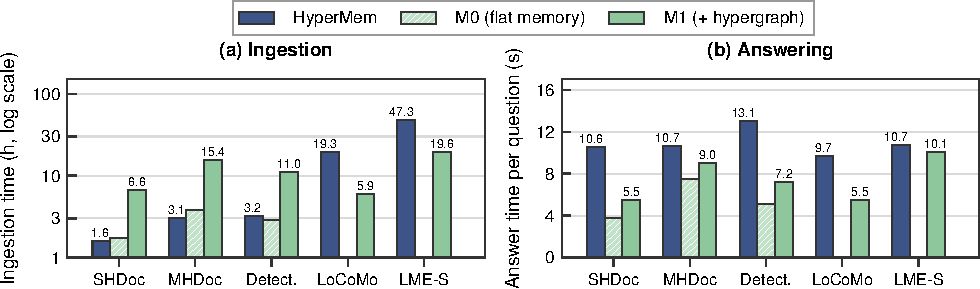
\includegraphics[width=\linewidth]{figures/results_cost.pdf}
\caption{Cost of user memory: (a) ingestion time and (b) answer time per question.}
\label{fig:res-cost}
\end{figure}
\paragraph{The available timings characterize M1, not the full M2 system.}
\Cref{fig:res-cost}b and \Cref{tab:eff-docqa} in the appendix show that M1 also has lower
answer latency than HyperMem on LoCoMo and \mbox{LongMemEval-S}, completing the five-benchmark latency
comparison. Its conversational ingestion time is lower as well, unlike the
document setting. These measurements are consistent with bounded graph access keeping answer
latency low, but they do not isolate the effects of candidate caps, model
calls, or execution conditions. M2 adds consolidation calls and can
change subsequent retrieval behavior. Its total ingestion cost, answer cost,
and graph reduction must be measured directly before attaching the M1
latency claims to the full system. Node and edge counts alone likewise do
not quantify evidence retention or compression.
\paragraph{Fewer agent steps do not necessarily mean fewer tokens.}
\Cref{tab:agent-token-consumption} separates the cost of learning a procedure from the
cost of applying it, with the token accounting given in \Cref{app:results-cost}. On WebShop, \ours uses the fewest
training and test tokens among the memory methods, 1.815M and 4.975M per run,
while achieving the highest mean success. On ALFWorld, its 3.813M test tokens
are the highest among the memory methods despite its lower mean step count.
A retrieved procedure can reduce interaction steps while increasing the
context processed at each step. Relative to no memory, test tokens rise on
both benchmarks, so procedural memory should be judged by the resulting
success and reuse, rather than assumed to save tokens automatically.
The reported totals do not determine how many future tasks are needed to
amortize memory learning, because no varying-horizon cost study is included.

\begin{table*}[tb]
\centering
\caption{Token use per run and success with GPT-6 Luna, mean $\pm$ std over three runs. Bold marks the best of the three memory methods.}
\label{tab:agent-token-consumption}
\small
\setlength{\tabcolsep}{7pt}
\begin{tabular}{llccc}
\toprule
Benchmark & Method
& Training tokens (M) $\downarrow$
& Test tokens (M) $\downarrow$
& Success rate (\%) $\uparrow$ \\
\midrule
\multirow{4}{*}{ALFWorld}
& No memory
& 0
& 2.147$\pm$0.048
& 69.4$\pm$0.7 \\
& ReasoningBank
& \textbf{1.747$\pm$0.122}
& \textbf{3.351$\pm$0.045}
& 66.9$\pm$2.8 \\
& AWM
& 2.749$\pm$0.059
& 3.674$\pm$0.332
& 73.6$\pm$1.9 \\
& \ours
& 2.253$\pm$0.100
& 3.813$\pm$0.490
& \textbf{76.4$\pm$6.2} \\
\midrule
\multirow{4}{*}{WebShop}
& No memory
& 0
& 4.238$\pm$0.463
& 31.9$\pm$1.8 \\
& ReasoningBank
& 2.010$\pm$0.242
& 6.620$\pm$0.674
& 25.7$\pm$3.8 \\
& AWM
& 1.909$\pm$0.127
& 5.448$\pm$0.356
& 36.0$\pm$4.3 \\
& \ours
& \textbf{1.815$\pm$0.054}
& \textbf{4.975$\pm$0.340}
& \textbf{37.4$\pm$2.1} \\
\bottomrule
\end{tabular}
\end{table*}


\subsection{What the experiments establish}
\label{sec:exp-discussion}

The results support the three properties in different measure. Accuracy has
the broadest support. The M0, M1, and M2 ordering holds on both conversational
benchmarks, and \ours leads the compared systems on four of the five QA
benchmarks, two of them with AutoDream disabled. As procedural memory, it has
the highest mean success among the compared memory methods on ALFWorld with
both backbones and on WebShop, and the highest MetaClaw-Bench score with both
backbones, while the no-memory comparisons show that retrieved experience can
also hurt. Efficiency holds for answering more than for ingestion. With
AutoDream disabled, \ours answers faster than HyperMem on every timed
benchmark, and on WebShop it uses the fewest training and test tokens among
the memory methods. Graph construction, however, makes document ingestion 3.8
to 4.0 times slower than flat memory, and the ALFWorld test tokens of \ours are
the highest among the memory methods. Practicality rests on the design and on
our protocol rather than on a deployment. One store serves both uses, no model
is fine-tuned, and every graph fact returned to the answerer cites its source
rows.

The tables evaluate complete configurations, so the component explanations in
this section remain interpretations, and the limitations in
\Cref{sec:conclusion} list the ablations that would test them. The tables also
do not measure merge precision, source-detail retention, skill provenance
coverage, or the contribution of the six-writer routing policy, and they do not
report memory length or user-memory ingestion tokens, for which graph counts
and answer tokens cannot substitute.
